\chapter{Implementation of a modular and scalable solution}
\sloppy

Se il capitolo precedente ha descritto in dettaglio i requisiti e il nuovo progetto architetturale per il nuovo sistema ServiceRequestManager (SRM), proponendo soluzioni mirate per superare le varie limitazioni tecnologiche e strutturali del sistema legacy SRP, questo capitolo segna il passaggio dal piano teorico alla realizzazione pratica, concentrandosi sull'implementazione concreta di una soluzione modulare e scalabile. 

Il focus primario di questa implementazione risiede nel modo in cui sono state risolte le sfide critiche descritte nei capitoli precedenti. Nello specifico si evidenzierà come la centralizzazione della logica di gestione e configurazione dei campi (e più in generale del catalogo) sul backend abbia eliminato il frontend monolitico e reso possibile un sistema di configurazione a tre livelli altamente riutilizzabile. Si illustrerà inotlre l'integrazione del nuovo flusso di esecuzione e retrieve delle anagrafiche tramite sistema di code di messaggi, essenziale per l'eliminazione della dipendenza dall'obsoleto SRP Agent.

\section{Automation of the Development Lifecycle through CI/CD Integration} 
% oppure DevOps Workflow Integration within the Developed System}

Per ogni funzionalità o modifica significativa del codice, viene creato un branch dedicato denominato con l'ID del ticket associato alla modifica (es: IN-7835). Questi branch sono utilizzati per lo sviluppo isolato delle nuove funzionalità, permettendo ai team di lavorare in parallelo senza interferenze. Una volta completata la modifica, il branch viene sottoposto a revisione del codice e test automatici tramite la pipeline CI/CD prima di essere integrato nel branch principale (main).

Esistono 3 ambienti live distinti: \texttt{devel}, \texttt{quality} e \texttt{production}. Il Git workflow aziendale prevede che i branch di funzionalità vengano prima mergiati in \texttt{devel} per ulteriori test e integrazioni, e successivamente in \texttt{quality} per la validazione finale prima del rilascio in produzione. Questo approccio garantisce che ogni modifica sia accuratamente verificata e testata in ambienti progressivamente più vicini alla produzione, riducendo il rischio di introdurre bug o regressioni nel sistema live. 

\subsection{Feat Branches}
Per i feat branches, la pipeline CI/CD è progettata per eseguire una serie di controlli automatici volti a garantire la qualità, la sicurezza e la conformità del codice prima della sua integrazione nei branch principali, non includendo quindi le fasi di build, test e deploy dell'applicativo, come mostrato in figura \ref{fig:feat-pipeline-workflow}.

\begin{figure}[htbp]
    \centering
    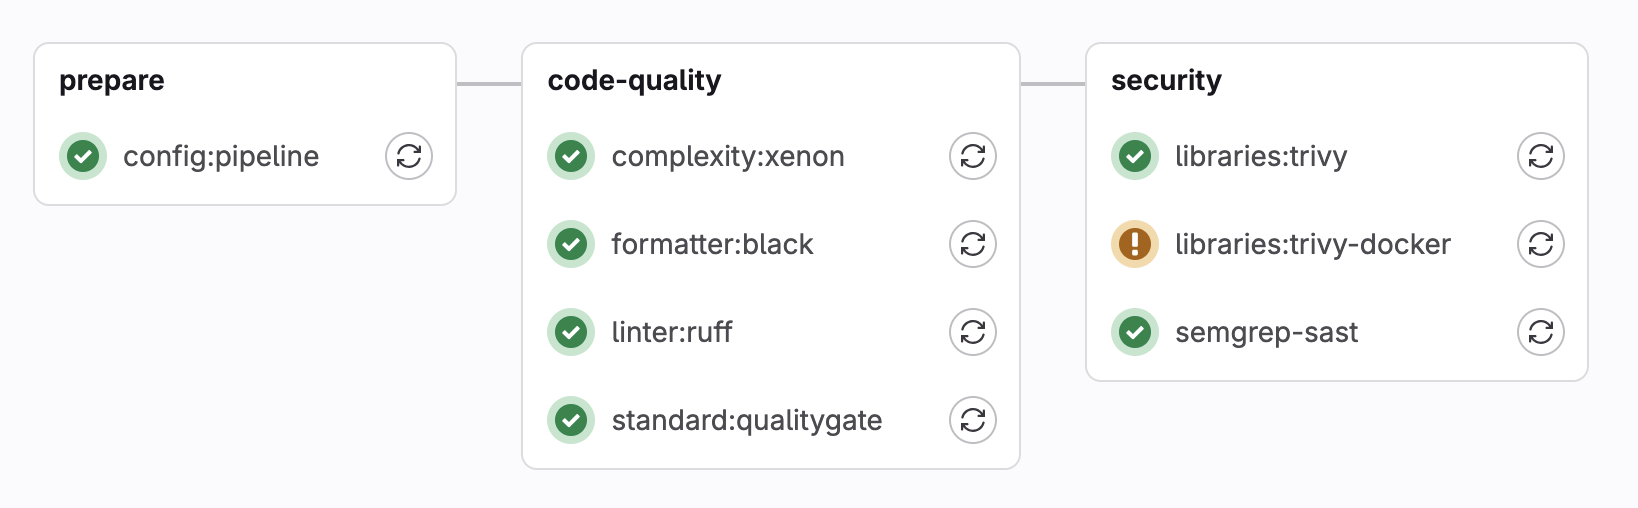
\includegraphics[width=\textwidth]{images/ci-cd/feat pipeline.png}
    \caption{Feat Branches pipeline workflow}
    \label{fig:feat-pipeline-workflow}
\end{figure}

\subsubsection{Prepare}
Lo stage \texttt{config:pipeline} ha il compito di preparare l'ambiente di esecuzione recuperando dinamicamente la configurazione del progetto da un servizio esterno. Dopo aver installato gli strumenti necessari, esegue una richiesta HTTP per ottenere i parametri di configurazione in formato JSON e li converte in variabili d'ambiente standardizzate, salvandole in un file .env. Tale file viene poi pubblicato come \textit{artifact}, in modo che gli step successivi della pipeline possano utilizzare queste informazioni per adattare il proprio comportamento alle impostazioni specifiche del progetto.
    
\subsubsection{Code Quality}
\paragraph{Complexity Check}
Lo stage \texttt{complexity:xenon} si occupa di misurare la complessità del codice tramite l'analizzatore statico \textit{Xenon}, con l'obiettivo di identificare file o funzioni che potrebbero risultare difficili da manutenere. Dopo aver predisposto l'ambiente Python ed installato lo strumento necessario, il job esegue l'analisi confrontando i risultati con una soglia di qualità predefinita. L'esito viene salvato in un file di report e inviato al sistema di monitoraggio della qualità del progetto. Se vengono rilevate criticità che superano il livello consentito, il job segnala un fallimento, contribuendo così a mantenere la complessità del software entro limiti sostenibili nel tempo.

\paragraph{Code Formatter}
Lo stage \texttt{formatter:black} ha lo scopo di verificare che il codice Python rispetti le convenzioni di formattazione stabilite dal progetto (PEP-8), utilizzando lo strumento \textit{Black}. Durante il job viene scaricata la configurazione di formattazione condivisa, quindi viene eseguito un controllo sull'intero repository senza applicare modifiche automatiche. L'esito dell'analisi viene salvato in un report e registrato nel sistema di monitoraggio della qualità. Se vengono trovati file non conformi allo stile richiesto, il job segnala un errore così da garantire che tutte le modifiche rispettino standard uniformi di formattazione del codice.

\paragraph{Code Linter}
Lo stage \texttt{linter:ruff} è dedicato al controllo statico del codice al fine di individuare errori, costruzioni poco sicure o non conformi alle linee guida interne di sviluppo. Viene eseguito un linter Python (\textit{Ruff}) che analizza l'intero progetto e produce un report con eventuali violazioni o segnalazioni di refactoring. I risultati vengono raccolti ed inviati al sistema di monitoraggio della qualità, contribuendo a mantenere uno stile uniforme e a prevenire potenziali problemi in fase di esecuzione. In caso di errori considerati bloccanti secondo le regole definite dal progetto, il job fallisce, impedendo l'integrazione di codice non conforme.

\paragraph{Quality Gate}
Lo stage \texttt{standard:qualitygate} analizza staticamente il progetto attraverso un insieme di regole che verificano la conformità agli standard aziendali. Il sistema ispeziona file Python, configurazioni YAML, requirements e script di deployment, controllando aspetti come la corretta configurazione del debug, la presenza di sistemi di monitoring (\textit{Sensu} / \textit{Prometheus}), l'utilizzo appropriato delle librerie standard aziendali, la configurazione dell'APM (Application Performance Monitoring), e la gestione sicura delle variabili d'ambiente. Ogni violazione delle regole viene riportata con dettagli sul file e la linea interessata, bloccando la pipeline se vengono rilevati errori critici. Questo approccio garantisce che solo codice conforme agli standard di sicurezza e qualità possa essere deployato in produzione, riducendo significativamente il rischio di problemi operativi e vulnerabilità.

\subsubsection{Security}
\paragraph{Libraries}
Lo stage \texttt{libraries:trivy} è focalizzato sull'analisi delle dipendenze allo scopo di individuare vulnerabilità note nei pacchetti utilizzati dal progetto. Viene utilizzato Trivy, un tool specializzato nella scansione di librerie e componenti software rispetto a database aggiornati di CVE \cite{trivy}. Il risultato del controllo permette di identificare tempestivamente rischi di sicurezza legati a versioni affette da bug o falle note \cite{trivy}, contribuendo così a mantenere un livello di sicurezza adeguato e a prevenire l'introduzione di dipendenze vulnerabili nel processo di rilascio.

Lo stage \texttt{libraries:trivy-docker}, invece, si focalizza sulla ricerca di misconfigurazioni nei file di deployment, Dockerfile e manifesti Kubernetes. Trivy esegue una scansione completa utilizzando una priorità di detection "\textit{comprehensive}" e genera un report dettagliato in formato JSON, che viene salvato come artifact per permettere analisi successive. La scansione verifica anche le licenze delle dipendenze e fallisce se vengono rilevate vulnerabilità critiche non risolte o misconfigurazioni significative. 

Questi due stage forniscono un feedback essenziale sulla postura di sicurezza del progetto, permettendo al team di identificare e correggere proattivamente potenziali problemi di sicurezza prima del deployment in produzione.

\paragraph{Static Application Security Testing (SAST)}
Questo stage esegue un'analisi statica del codice sorgente per identificare vulnerabilità di sicurezza e pattern di codice potenzialmente pericolosi. \textit{Semgrep} analizza il codice senza eseguirlo, rilevando problematiche come SQL injection, XSS, gestione insicura di credenziali e altre vulnerabilità OWASP \cite{semgrep}. Lo stage genera un report standardizzato in formato JSON che classifica le vulnerabilità per severity (Critical, Medium, Info) e include metadati come SHA del commit, branch e nome del progetto. Per i branch principali (quality, devel, master), i risultati vengono inviati a un sistema centralizzato di valutazione dei progetti per il tracking storico. In questo modo, si garantisce che nessun codice con problemi di sicurezza noti possa raggiungere gli ambienti di produzione.

\subsection{Live Environment Branches}
Per gli ambienti live, ovvero quelli di devel, quality e production, la pipeline CI/CD include ulteriori fasi specifiche per la build, il test e il deploy dell'applicativo, come mostrato in figura \ref{fig:live-env-pipeline-workflow}, escludendo le fasi già coperte per i feat branches.
 
\begin{figure}[htbp]
    \centering
    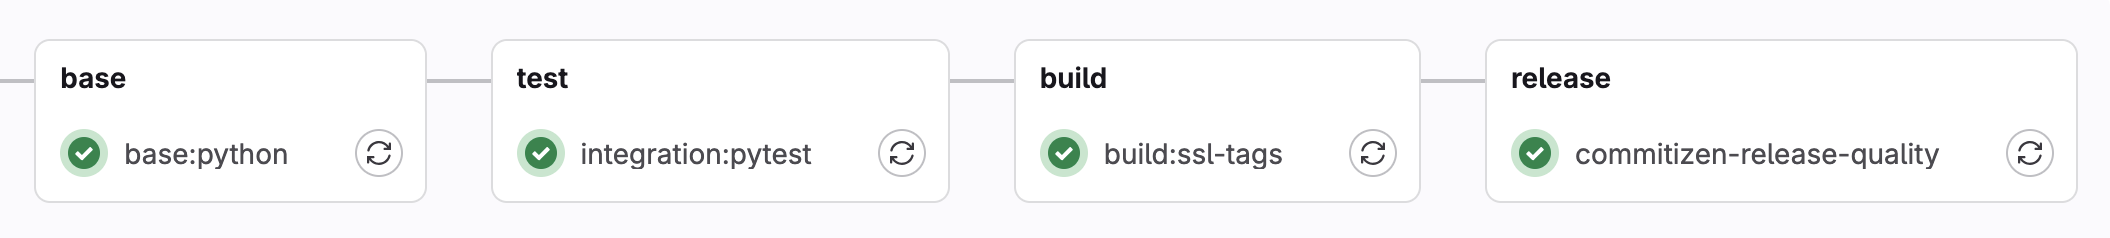
\includegraphics[width=\textwidth]{images/ci-cd/live env pipeline.png}
    \caption{Live Environment Branches pipeline workflow (ecluding already covered stages)}
    \label{fig:live-env-pipeline-workflow}
\end{figure}

\subsubsection{Base Image Build}
Lo stage \texttt{base:python} è responsabile della costruzione dell'immagine Docker di base del progetto, contenente tutte le dipendenze Python definite nel file \texttt{requirements.txt}. 

Questo stage implementa una strategia di build ottimizzata attraverso la separazione in layer: l'immagine viene ricostruita solamente quando vengono rilevate modifiche nei file \texttt{requirements.txt} o \texttt{Dockerfile\_base}, evitando rebuild non necessari e riducendo significativamente i tempi di esecuzione della pipeline. Il job viene eseguito esclusivamente sui branch principali (devel, quality, master). 

Questa separazione in tre Dockerfile distinti (Dockerfile, Dockerfile\_base, Dockerfile\_ssl) consente di sfruttare la cache Docker in modo intelligente: se le dipendenze non cambiano, gli stage successivi possono riutilizzare l'immagine base esistente, velocizzando notevolmente il processo di build e riducendo il carico sui runners CI/CD.

\subsubsection{Test}
Lo stage \texttt{test:pytest} si occupa dell'esecuzione della suite di test automatizzati del progetto utilizzando PyTest e PostgreSQL come database di riferimento. Il job configura un ambiente di test isolato avviando un'istanza dedicata di PostgreSQL 16 come servizio containerizzato, con credenziali e parametri di connessione definiti dinamicamente attraverso variabili d'ambiente. L'esecuzione dei test avviene solo se è presente il file requirements\_tests.txt e viene adattata in base al contesto: per i branch devel e quality vengono utilizzate rispettivamente le immagini Docker \texttt{devel-latest} e \texttt{quality-latest}, mentre per le merge request viene impiegata l'immagine \texttt{production-latest}, garantendo così che i test vengano eseguiti in condizioni quanto più simili all'ambiente target. 

Lo stage implementa inoltre un controllo rigoroso sulla copertura del codice: se la percentuale di coverage risulta inferiore all'80\%, la pipeline fallisce automaticamente, garantendo che venga mantenuto un livello minimo di qualità e affidabilità del software attraverso una adeguata copertura dei test. Lo stage viene escluso dai tag e dal branch master per evitare esecuzioni ridondanti. 

Questo approccio assicura che ogni modifica al codice venga validata contro un database reale prima dell'integrazione, riducendo il rischio di regressioni e problemi di compatibilità.

\subsubsection{SSL Image Build}
Lo stage \texttt{build:ssl-tags} è dedicato alla costruzione dell'immagine Docker intermedia contenente i certificati SSL e le configurazioni di sicurezza necessarie per le comunicazioni crittografate del progetto. Questo stage fa parte della strategia di build multi-layer e viene eseguito esclusivamente sui branch quality e master, solo se presente il file \texttt{Dockerfile\_ssl}. Analogamente allo stage \texttt{base:python}, implementa un sistema di rebuild condizionale che ricostruisce l'immagine solamente quando vengono rilevate modifiche nei file \texttt{requirements.txt} o \texttt{Dockerfile\_ssl}, ottimizzando i tempi di esecuzione della pipeline attraverso il riutilizzo della cache Docker. 

Questa separazione del layer SSL consente di gestire in modo indipendente le configurazioni di sicurezza e i certificati, facilitando gli aggiornamenti e la manutenzione degli aspetti legati alla crittografia senza dover ricostruire l'intera immagine applicativa.

\subsubsection{Release}
Lo stage \texttt{commitizen-release} gestisce il processo di versioning automatico e la creazione di release del progetto utilizzando \textit{Commitizen}, uno strumento che analizza la cronologia dei commit per determinare automaticamente il numero di versione secondo le convenzioni di Semantic Versioning\footnote{Il semantic versioning è una convenzione di versionamento che adotta lo schema MAJOR.MINOR.PATCH, dove il numero MAJOR viene incrementato in caso di modifiche incompatibili con le versioni precedenti, il numero MINOR in seguito all'introduzione di funzionalità compatibili, e il numero PATCH per interventi correttivi che non alterano le funzionalità esistenti.} e Conventional Commit\footnote{Il Conventional Commits è una convenzione per la stesura dei messaggi di commit che utilizza una struttura standardizzata  composta da un tipo di modifica (feat, fix, chore, test, refactor, ...), un oggetto opzionale e una descrizione, al fine di rendere più chiaro e automatizzabile il tracciamento delle modifiche, la generazione delle note di rilascio e il versionamento del software.}. Lo stage \texttt{commitizen-release} opera sul branch master e, dopo aver configurato le credenziali Git e sincronizzato il repository locale con quello remoto, esegue un bump automatico della versione basandosi sui messaggi dei commit convenzionali (feat, fix, core, refactor, test, ...). Il processo crea automaticamente i tag Git corrispondenti e li pusha al repository con l'opzione \texttt{ci.skip} per evitare l'attivazione ricorsiva della pipeline. Lo stage \texttt{commitizen-release-quality} funziona in modo analogo ma è dedicato al branch quality e genera versioni pre-release con suffisso "alpha", modificando dinamicamente la configurazione di Commitizen per adattarla al contesto di test. Entrambi gli stage vengono eseguiti solo se è presente il file di configurazione \texttt{.cz.yaml} e sono esclusi dalle merge request, garantendo che il versioning avvenga esclusivamente sui branch principali dopo l'integrazione del codice. 

Questo approccio automatizzato elimina la necessità di gestire manualmente i numeri di versione e assicura coerenza e tracciabilità nel processo di rilascio del software.

\subsection{Tag Branches}
\begin{figure}[htbp]
    \centering
    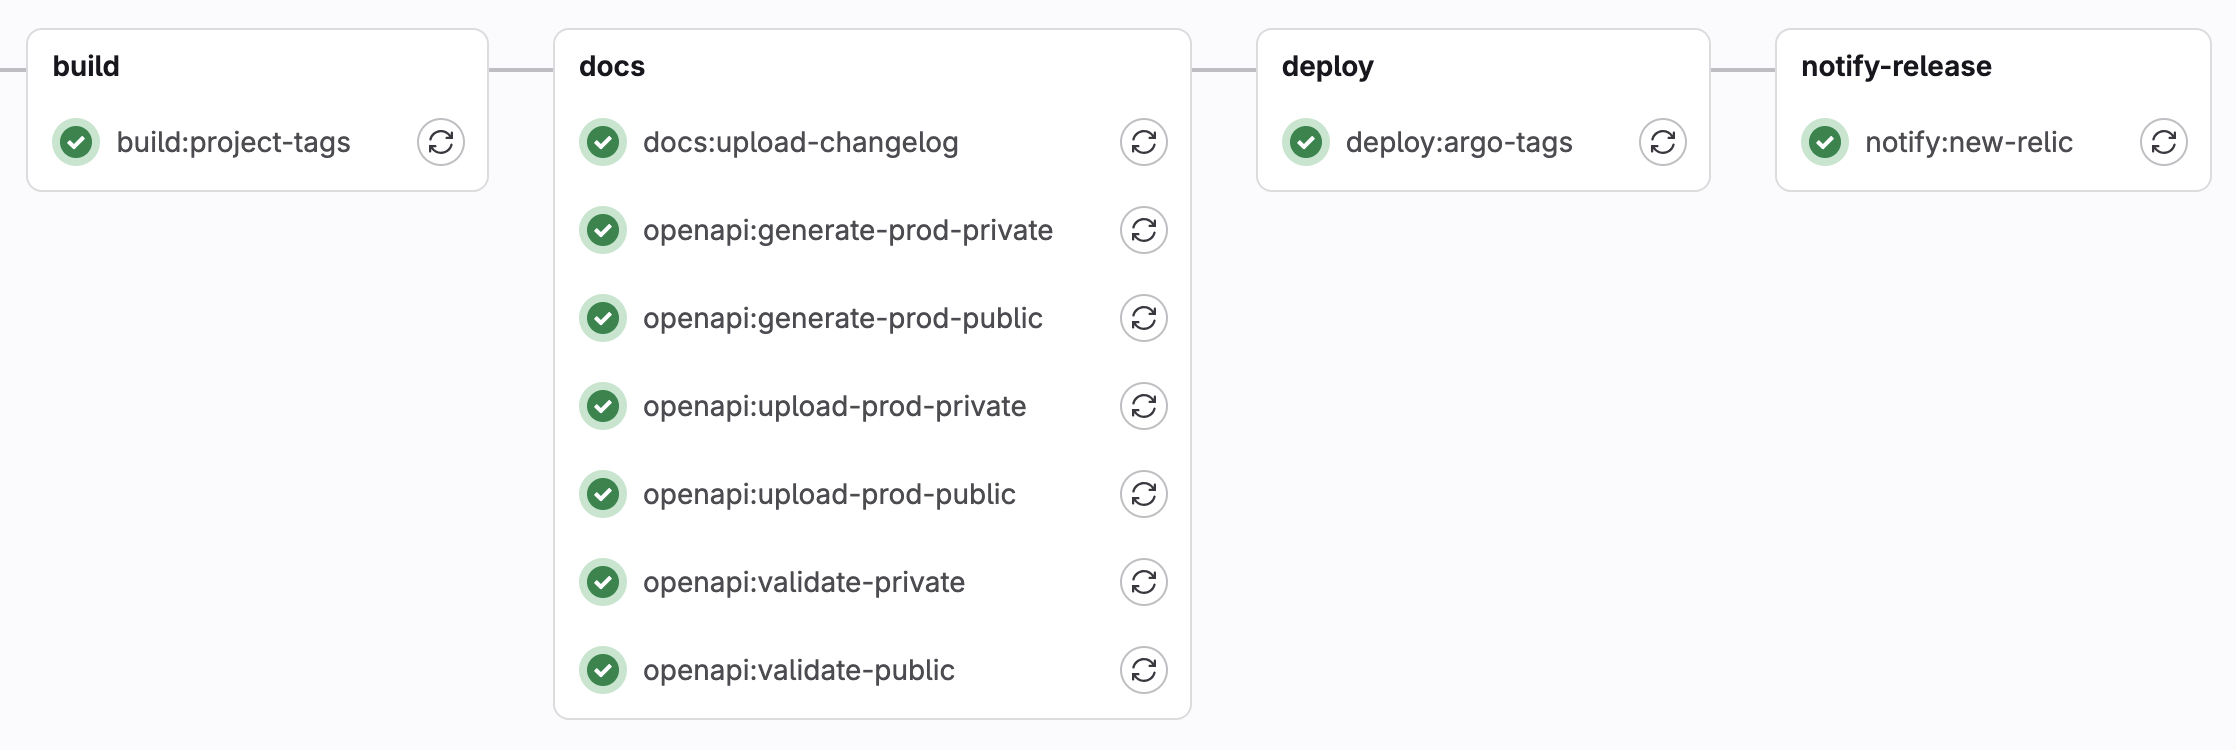
\includegraphics[width=\textwidth]{images/ci-cd/tag pipeline.png}
    \caption{Tag Branches pipeline workflow (ecluding already covered stages)}
    \label{fig:tags-pipeline-workflow}
\end{figure}

\subsubsection{Project Build}
Lo stage \texttt{build:project-tags} rappresenta la fase conclusiva del processo di build, responsabile della costruzione dell'immagine Docker finale dell'applicazione pronta per il deployment. Questo stage viene attivato esclusivamente quando viene creato un tag Git che rispetta il formato Semantic Versioning (major.minor.patch), garantendo che solo versioni formalmente rilasciate vengano containerizzate. Il job utilizza il \texttt{Dockerfile} principale, che assembla tutti i layer precedentemente costruiti (base e SSL), aggiungendo il codice applicativo e le configurazioni finali. Lo stage implementa una logica condizionale che previene l'esecuzione se esiste un \texttt{Dockerfile\_base} separato, delegando in quel caso la build a flussi più ottimizzati che sfruttano la cache multi-layer. L'immagine risultante viene taggata con la versione specifica del rilascio e pubblicata nel registry Docker aziendale, costituendo l'artifact definitivo pronto per essere deployato negli ambienti di produzione attraverso gli stage successivi della pipeline.

\subsubsection{Docs}
Gli stage di documentazione automatizzano la generazione e la pubblicazione della documentazione tecnica del progetto. Lo stage \texttt{docs:upload-changelog} si occupa di pubblicare il changelog su Techpedia, una  piattaforma aziendale di documentazione collaborativa, utilizzando l'API GraphQL per creare o aggiornare automaticamente le pagine di changelog quando viene creato un nuovo tag di release. Gli stage \texttt{openapi:generate} si occupano invece della generazione della documentazione API in formato OpenAPI/Swagger, utilizzando il framework Django Spectacular per estrarre la specifica dalle annotazioni del codice. Questi stage producono due versioni della documentazione: una pubblica, contenente solo gli endpoint accessibili esternamente, e una privata con la documentazione completa di tutte le API interne. La generazione avviene per ciascun ambiente (production e quality) collegandosi ai rispettivi database per garantire che la documentazione rifletta accuratamente la struttura dati effettiva. Gli schemi OpenAPI generati vengono salvati come artifact e possono essere successivamente utilizzati per la validazione automatica, la generazione di client SDK o la pubblicazione su portali di documentazione API, garantendo che la documentazione tecnica sia sempre sincronizzata con il codice e accessibile agli sviluppatori e ai consumatori delle API.

\subsubsection{Deploy with ArgocD}
Gli stage \texttt{deploy:argo-tags} e \texttt{deploy:argo-tags-quality} gestiscono il deployment automatico dell'applicazione sugli ambienti Kubernetes attraverso ArgoCD\footnote{ArgoCD è uno strumento di GitOps per Kubernetes che mantiene automaticamente lo stato delle applicazioni nel cluster sincronizzato con quello dichiarato su Git.}. Lo stage \texttt{deploy:argo-tags} si attiva esclusivamente per tag di release stable (formato major.minor.patch) ed effettua il deployment in ambiente di produzione, mentre \texttt{deploy:argo-tags-quality} gestisce le versioni pre-release (con suffissi alpha, beta, rc) deployandole nell'ambiente quality per test di integrazione e validazione. Entrambi gli stage utilizzano un'immagine Docker specializzata che contiene candymand, uno strumento wrapper sviluppato internamente che interagisce con ArgoCD per automatizzare il processo di deployment dichiarativo. Il tool riceve come parametri il namespace del progetto e la versione da deployare, quindi aggiorna automaticamente le configurazioni Git dei manifest Kubernetes, innescando il processo di GitOps gestito da ArgoCD che sincronizza lo stato desiderato con il cluster. Questo approccio garantisce deployment completamente tracciabili, rollback semplificati e piena aderenza ai principi di Infrastructure as Code, eliminando interventi manuali e riducendo il rischio di errori durante il rilascio.

\subsubsection{Notify Release}
Lo stage \texttt{notify:new-relic} si occupa di registrare automaticamente le nuove release dell'applicazione sulla piattaforma di Application Performance Monitoring \textit{New Relic}, creando un marker di deployment che facilita la correlazione tra versioni del software e metriche di performance. Il job viene attivato per qualsiasi tag che rispetti il formato Semantic Versioning e utilizza l'API GraphQL di New Relic per identificare l'applicazione corretta tramite il suo GUID, distinguendo automaticamente tra l'istanza di produzione e quella di quality in base alla presenza o meno di suffissi pre-release nel tag. Una volta identificata l'entità monitorata, lo stage crea un evento di change tracking che registra la versione deployata, consentendo agli operatori e ai team di development di visualizzare nei dashboard di New Relic quando sono avvenuti i deployment e di correlare eventuali anomalie nelle performance o negli errori con specifiche versioni del software. Questo meccanismo di notifica automatica elimina la necessità di registrazione manuale dei deployment e fornisce una visibilità completa sul ciclo di vita dell'applicazione, supportando attività di troubleshooting, analisi di regressioni e valutazione dell'impatto delle release sulla stabilità del sistema.

\section{Implementation of the Deployment Architecture on Kubernetes}

\section{Backend Service Implementation}

\subsection{Technological Overview}

\subsection{Catalog Management}

\subsection{Message Queue System for Asynchronous Execution Flow}

\subsection{Implementation of Customers' Master Data Import}

\subsection{Logging and Monitoring}

\section{Frontend Application Implementation}

\subsection{Technological Overview}

\subsection{Service Request Creation Platform for End Users}

\subsection{Administrative Configuration Platform for System Administrators}
